\documentclass[letter,12pt]{article}
\usepackage[paperheight=27.94cm,paperwidth=21.59cm,bindingoffset=0in,left=3cm,right=2.0cm, top=3.5cm,bottom=2.5cm, headheight=200pt, headsep=1.0\baselineskip]{geometry}
\usepackage{graphicx,lastpage}
\usepackage{upgreek}
\usepackage{censor}
\usepackage[spanish,es-tabla]{babel}
\usepackage{pdfpages}
\usepackage{tabularx}
\usepackage{graphicx}
\usepackage{adjustbox}
\usepackage{xcolor}
\usepackage{colortbl}
\usepackage{rotating}
\usepackage{multirow}
\usepackage[utf8]{inputenc}
\usepackage{float}
\usepackage{hyperref}
\usepackage{listings}
\lstset{
    basicstyle=\small\ttfamily,
    breaklines=true,
    breakatwhitespace=false,
    columns=flexible,
    keepspaces=true,
    frame=single,
    xleftmargin=5pt,
    xrightmargin=5pt,
}

\renewcommand{\tablename}{Tabla}
\usepackage{fancyhdr}
\pagestyle{fancy}


%
\begin{document}
%
   \title{\Huge{Informe Laboratorio 5}}

   \author{\textbf{Sección 1} \\  \\Alumno Felipe Maturana \\ e-mail: felipe.maturana1@mail.udp.cl}
          
   \date{Junio 2026}

   \maketitle

   \newpage
   
   \tableofcontents
 
  \newpage
  

\section*{Descripción de actividades}
\addcontentsline{toc}{section}{Descripción de actividades}
Para este último laboratorio, se solicita trabajar con Docker y el protocolo SSH, a fin de poder entender el concepto de cripografía asimétrica y firmas digitales.\\

Para lo anterior deberá:

\begin{itemize}
    \item Crear 4 contenedores en Docker por medio de un DockerFile, donde cada uno tendrá el siguiente SO:
        Ubuntu 16.10, Ubuntu 18.10, Ubuntu 20.10 y Ubuntu 22.10 a los cuales se llamarán C1, C2, C3 y C4 respectivamente.\\
        El equipo con Ubuntu 22.10 también será utilizado como S1.
        
    \item  Para cada uno de ellos, deberá instalar el cliente openSSH disponible en los repositorios de apt, y para el equipo S1 deberá también instalar el servidor openSSH.

    \item En S1 deberá crear el usuario \textquotedblleft\textbf{prueba}\textquotedblright con contraseña \textquotedblleft\textbf{prueba}\textquotedblright, para acceder a él desde los clientes por el protocolo SSH.
    
    \item En total serán 4 escenarios, donde cada uno corresponderá a los siguientes equipos:
    \begin{itemize}
        \item C1 $\rightarrow$ S1
        \item C2 $\rightarrow$ S1
        \item C3 $\rightarrow$ S1
        \item C4 $\rightarrow$ S1
    \end{itemize}
\end{itemize}

Pasos:

\begin{enumerate}
\item Para cada uno de los 4 escenarios, deberá capturar el tráfico generado por cada conexión con el server. A partir de cada handshake, deberá analizar el patrón de tráfico generado por cada cliente y adicionalmente obtener el HASSH que lo identifique. De esta forma podrá obtener una huella digital para cada cliente a partir de su tráfico. Cada HASSH deberá compararlo con la base de datos HASSH disponible en el módulo de TLS, e identificar si el hash obtenido corresponde a la misma versión de su cliente.\\\\
Indique el tamaño de los paquetes del flujo generados por el cliente y el contenido asociado a cada uno de ellos. Indique qué información distinta contiene el escenario siguiente (diff incremental). El objetivo de este paso es identificar claramente los cambios entre las distintas versiones de ssh.\\

\newpage

\item Para poder identificar que el usuario efectivamente es el informante, éste utilizará una versión única de cliente. ¿Con qué cliente SSH se habrá generado el siguiente tráfico?

\begin{figure}[ht]
    \centering
    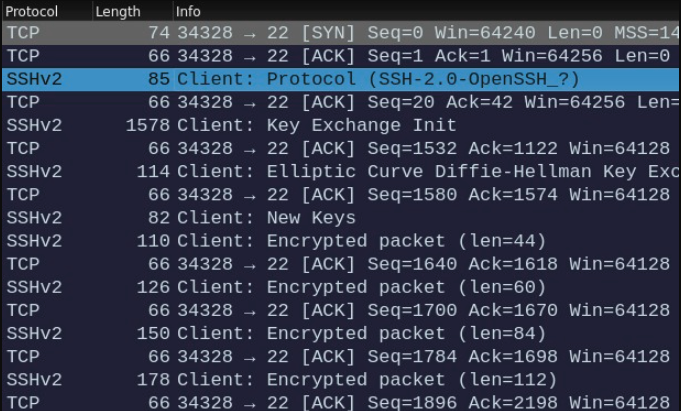
\includegraphics[width=1\linewidth]{Desarrollo/trafico.png}
    \caption{Tráfico generado del informante}
    \label{fig:trafico}
\end{figure}

Replique este tráfico generado en la imagen. Debe generar el tráfico con la misma versión resaltada en azul. Recuerde que toda la información generada es parte del sw, por lo tanto usted puede modificar toda la información.

\item Para que el informante esté seguro de nuestra identidad, nos pide que el patrón del tráfico de nuestro server también sea modificado, hasta que el Key Exchange Init del server sea menor a 300 bytes. Indique qué pasos realizó para lograr esto.

\begin{figure}[H]
    \centering
    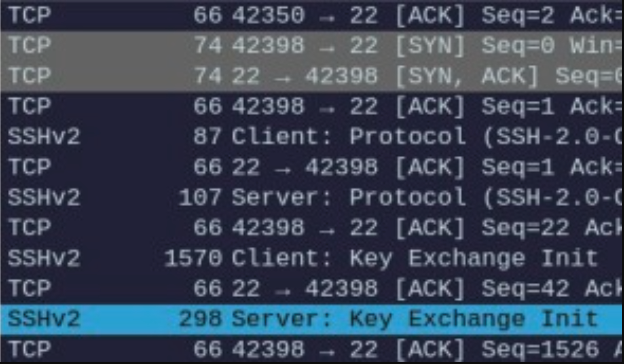
\includegraphics[width=1\linewidth]{Desarrollo/exchange.png}
    \caption{Captura del Key Exchange}
    \label{fig:exchange}
\end{figure}

\item Tomando en cuenta lo aprendido en este laboratorio, así como en los anteriores, explique el protocolo OpenSSH y las diferentes capas de seguridad que son parte del protocolo para garantizar los principios de seguridad de la información, integridad, confidencialidad, disponibilidad, autenticidad y no repudio. Es importante que sea muy específico en el objetivo del principio en el protocolo. En caso de considerar que alguno de los principios no se cumple, justifique su razonamiento. Es fundamental que su análisis se base en el tráfico SSH interceptado.

\end{enumerate}

\section{Desarrollo (Parte 1)}

\subsection{Códigos de cada Dockerfile}
Para realizar esta experiencia, se crearon cuatro Dockerfiles que instalan el cliente de OpenSSH en diferentes versiones de Ubuntu, además de configurar el servidor en la versión más reciente (C4/S1).

\subsubsection{C1}
\begin{lstlisting}
FROM ubuntu:16.10

# Adjust sources for EOL version
RUN sed -i -e 's/archive.ubuntu.com/old-releases.ubuntu.com/g' /etc/apt/sources.list && \
    sed -i -e 's/security.ubuntu.com/old-releases.ubuntu.com/g' /etc/apt/sources.list

RUN apt-get update && apt-get install -y \
    openssh-client \
    iputils-ping \
    tcpdump \
    && rm -rf /var/lib/apt/lists/*

CMD ["bash"]
\end{lstlisting}

\subsubsection{C2}
\begin{lstlisting}
FROM ubuntu:18.10

# Adjust sources for EOL version
RUN sed -i -e 's/archive.ubuntu.com/old-releases.ubuntu.com/g' /etc/apt/sources.list && \
    sed -i -e 's/security.ubuntu.com/old-releases.ubuntu.com/g' /etc/apt/sources.list

RUN apt-get update && apt-get install -y \
    openssh-client \
    iputils-ping \
    tcpdump \
    && rm -rf /var/lib/apt/lists/*

CMD ["bash"]
\end{lstlisting}

\subsubsection{C3}
\begin{lstlisting}
FROM ubuntu:20.10

# Adjust sources for EOL version
RUN sed -i -e 's/archive.ubuntu.com/old-releases.ubuntu.com/g' /etc/apt/sources.list && \
    sed -i -e 's/security.ubuntu.com/old-releases.ubuntu.com/g' /etc/apt/sources.list

RUN apt-get update && apt-get install -y \
    openssh-client \
    iputils-ping \
    tcpdump \
    && rm -rf /var/lib/apt/lists/*

CMD ["bash"]
\end{lstlisting}

\subsubsection{C4/S1}
\begin{lstlisting}
FROM ubuntu:22.10

# Adjust sources for EOL version
RUN sed -i -e 's/archive.ubuntu.com/old-releases.ubuntu.com/g' /etc/apt/sources.list && \
    sed -i -e 's/security.ubuntu.com/old-releases.ubuntu.com/g' /etc/apt/sources.list

RUN apt-get update && apt-get install -y \
    openssh-server \
    openssh-client \
    iputils-ping \
    tcpdump \
    && rm -rf /var/lib/apt/lists/*

# Create user 'prueba' with password 'prueba'
RUN useradd -m -s /bin/bash prueba && echo "prueba:prueba" | chpasswd

RUN mkdir -p /var/run/sshd

EXPOSE 22

CMD ["/usr/sbin/sshd", "-D"]
\end{lstlisting}

\subsubsection{Docker Compose}
\begin{lstlisting}
services:
  s1:
    build:
      context: ./C4
      network: host
    image: c4
    container_name: s1
    networks:
      ssh_net:
        ipv4_address: 172.21.0.10

  c1:
    build:
      context: ./C1
      network: host
    image: c1
    container_name: c1
    tty: true
    stdin_open: true
    depends_on:
      - s1
    networks:
      ssh_net:
        ipv4_address: 172.21.0.11

  c2:
    build:
      context: ./C2
      network: host
    image: c2
    container_name: c2
    tty: true
    stdin_open: true
    depends_on:
      - s1
    networks:
      ssh_net:
        ipv4_address: 172.21.0.12

  c3:
    build:
      context: ./C3
      network: host
    image: c3
    container_name: c3
    tty: true
    stdin_open: true
    depends_on:
      - s1
    networks:
      ssh_net:
        ipv4_address: 172.21.0.13

  c4:
    build:
      context: ./C4
      network: host
    image: c4
    container_name: c4_client
    depends_on:
      - s1
    networks:
      ssh_net:
        ipv4_address: 172.21.0.14

networks:
  ssh_net:
    driver: bridge
    ipam:
      config:
        - subnet: 172.21.0.0/24
\end{lstlisting}

\subsubsection{Comandos para levantar el entorno}
Para construir y levantar los contenedores se utilizó el siguiente comando desde el directorio \texttt{src}:
\begin{lstlisting}
docker compose up -d --build
\end{lstlisting}

\subsection{Creación de las credenciales para S1}
Para el servidor S1, la creación del usuario se configuró de manera automática directamente en su Dockerfile. Se utilizó el siguiente comando para crear el usuario \textbf{prueba} con la contraseña \textbf{prueba} y asignarles su directorio personal:

\begin{lstlisting}
RUN useradd -m -s /bin/bash prueba && echo "prueba:prueba" | chpasswd
\end{lstlisting}

\subsection{Tráfico generado por C1, detallando tamaño paquetes del flujo y el HASSH respectivo (detallado)}
Para el cliente C1 (Ubuntu 16.10), se capturó el flujo de tráfico hacia el servidor S1. El proceso de handshake se divide en las siguientes etapas principales:

\begin{itemize}
    \item \textbf{Protocol Exchange (Rojo)}: Intercambio de versiones de software entre cliente y servidor.
    \item \textbf{Key Exchange Init (Verde)}: Negociación de algoritmos de cifrado, compresión y hashing.
    \item \textbf{Elliptic Curve Diffie-Hellman (Naranjo)}: Proceso de generación y compartición de llaves para el canal seguro.
\end{itemize}

\begin{figure}[H]
    \centering
    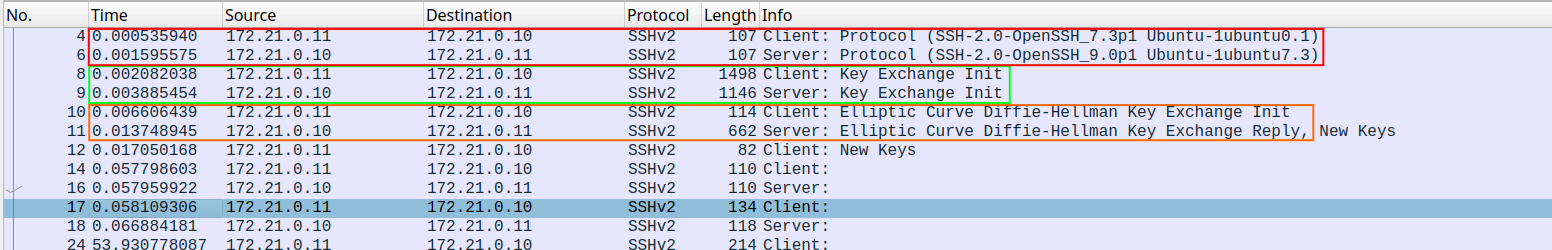
\includegraphics[width=0.8\linewidth]{analisis/1/packets_hassh_c1.png}
    \caption{Handshake detallado y captura de paquetes para C1}
\end{figure}

El primer paquete enviado por el cliente para la negociación (KEXINIT) tiene un tamaño de \textbf{1498 bytes}. A partir de los algoritmos propuestos por este cliente, se obtuvo el siguiente HASSH:

\begin{itemize}
    \item \textbf{HASSH}: \texttt{0e4584cb9f2dd077dbf8ba0df8112d8e}
\end{itemize}

\begin{figure}[H]
    \centering
    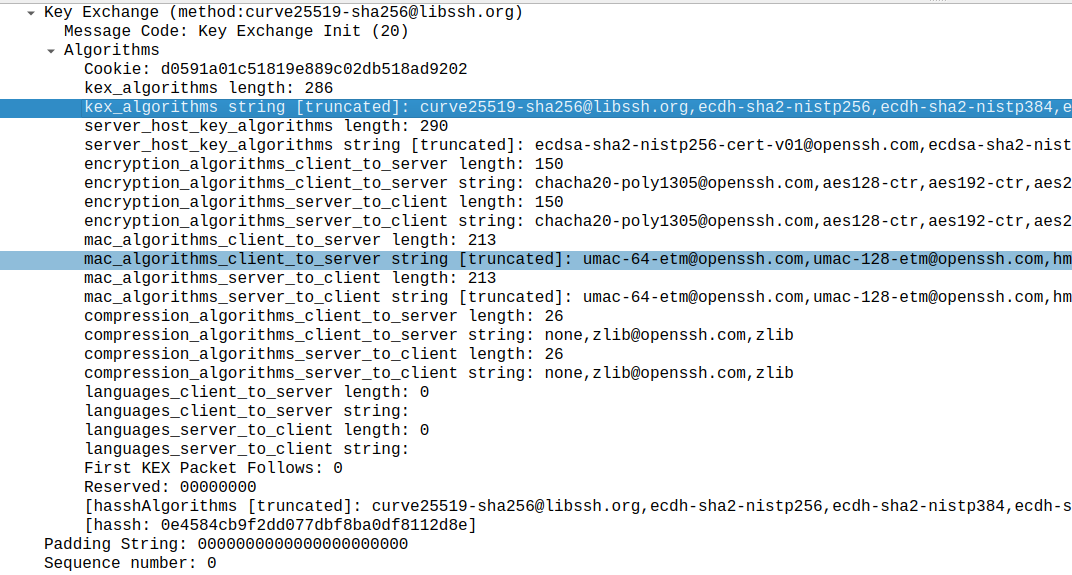
\includegraphics[width=0.8\linewidth]{analisis/1/key_exchange_c1.png}
    \caption{Detalle de algoritmos y HASSH para C1}
\end{figure}

\subsection{Tráfico generado por C2, detallando tamaño paquetes del flujo y el HASSH respectivo (detallado)}
Para el cliente C2 (Ubuntu 18.10), el proceso de handshake sigue la misma estructura lógica de intercambio de protocolos y negociación de llaves. En este escenario, el paquete KEXINIT presenta un tamaño de \textbf{1426 bytes}.

\begin{itemize}
    \item \textbf{HASSH}: \texttt{06046964c022c6407d15a27b12a6a4fb}
\end{itemize}

\begin{figure}[H]
    \centering
    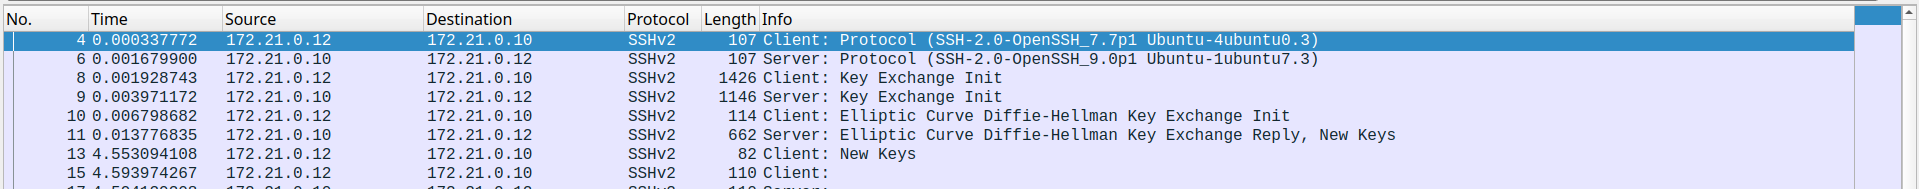
\includegraphics[width=0.8\linewidth]{analisis/1/packets_hassh_c2.png}
    \caption{Captura de paquetes para C2}
\end{figure}

\begin{figure}[H]
    \centering
    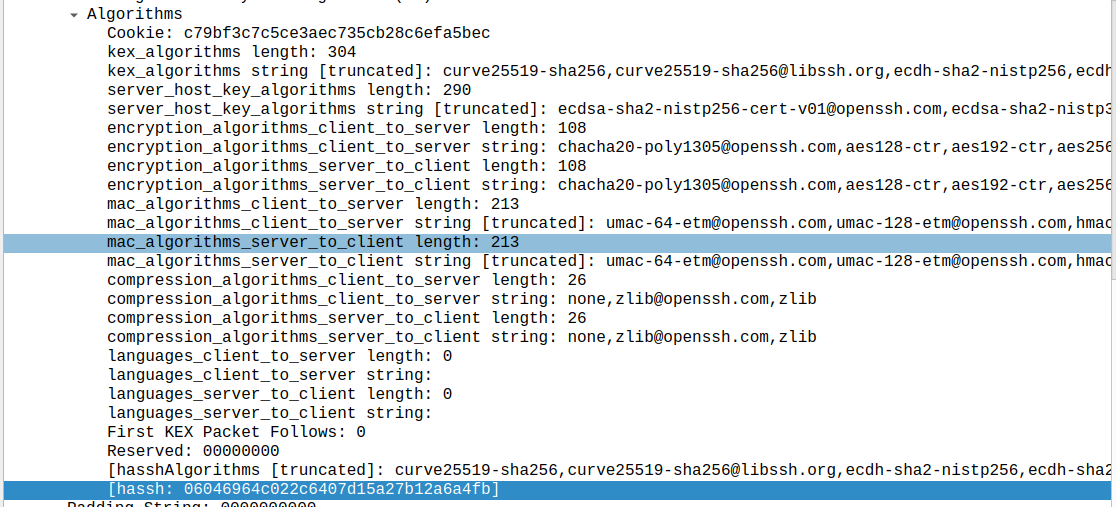
\includegraphics[width=0.8\linewidth]{analisis/1/key_exchange_c2.png}
    \caption{Detalle de algoritmos y HASSH para C2}
\end{figure}

\subsection{Tráfico generado por C3, detallando tamaño paquetes del flujo y el HASSH respectivo (detallado)}
El cliente C3 (Ubuntu 20.10) muestra un incremento en la complejidad de los algoritmos soportados. El tamaño del paquete KEXINIT es de \textbf{1578 bytes}, siendo el más extenso de los analizados hasta ahora debido a la inclusión de nuevos métodos de intercambio.

\begin{itemize}
    \item \textbf{HASSH}: \texttt{ae8bd7dd09970555aa4c6ed22adbbf56}
\end{itemize}

\begin{figure}[H]
    \centering
    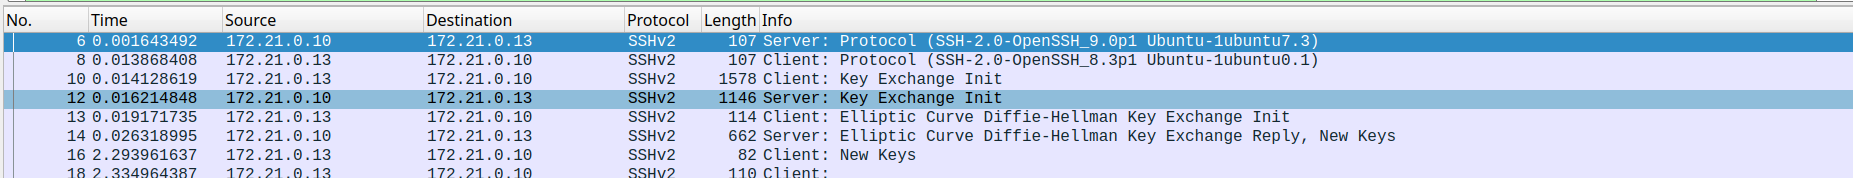
\includegraphics[width=0.8\linewidth]{analisis/1/packets_hassh_c3.png}
    \caption{Captura de paquetes para C3}
\end{figure}

\begin{figure}[H]
    \centering
    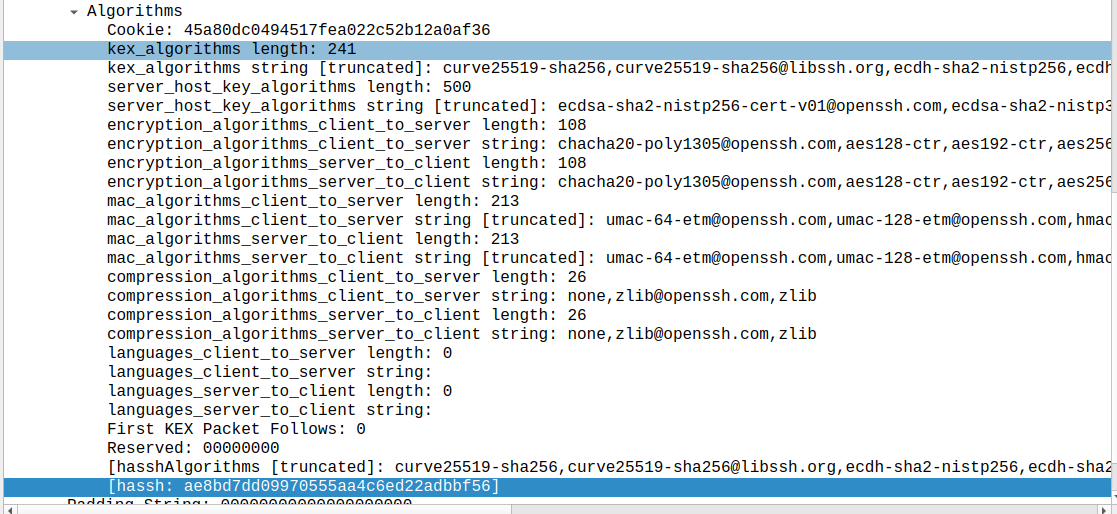
\includegraphics[width=0.8\linewidth]{analisis/1/key_exchange_c3.png}
    \caption{Detalle de algoritmos y HASSH para C3}
\end{figure}

\subsection{Tráfico generado por C4 (iface lo), detallando tamaño paquetes del flujo y el HASSH respectivo (detallado)}
Finalmente, para C4 (Ubuntu 22.10), el paquete KEXINIT tiene un tamaño de \textbf{1570 bytes}. Se observa la presencia de algoritmos modernos como \texttt{sntrup761x25519-sha512@openssh.com}.

\begin{itemize}
    \item \textbf{HASSH}: \texttt{78c05d999799066a2b4554ce7b1585a6}
\end{itemize}

\begin{figure}[H]
    \centering
    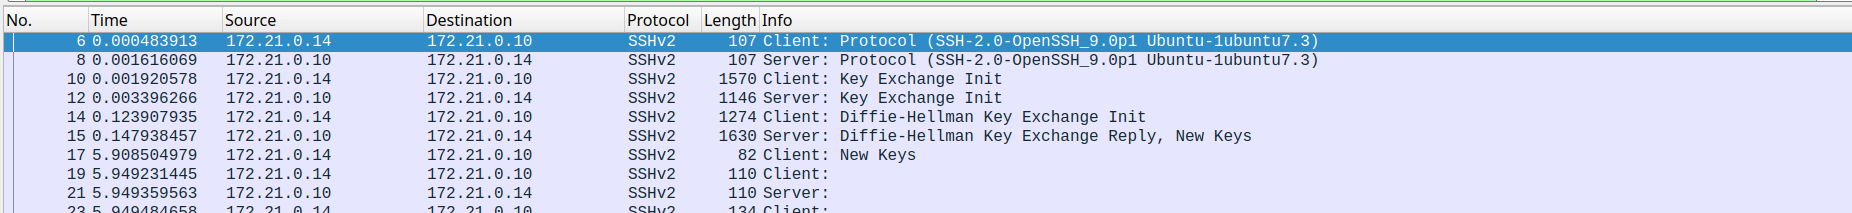
\includegraphics[width=0.8\linewidth]{analisis/1/packets_hassh_c4.png}
    \caption{Captura de paquetes para C4}
\end{figure}

\begin{figure}[H]
    \centering
    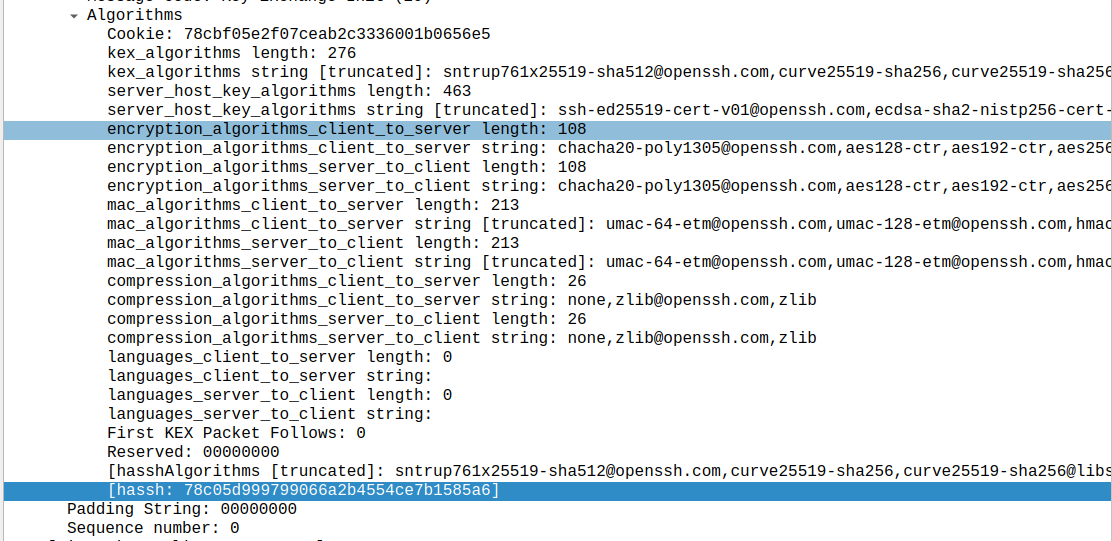
\includegraphics[width=0.8\linewidth]{analisis/1/key_exchange_c4.png}
    \caption{Detalle de algoritmos y HASSH para C4}
\end{figure}

\subsection{Compara la versión de HASSH obtenida con la base de datos para validar si el cliente corresponde al mismo}

\subsection{Tipo de información contenida en cada uno de los paquetes generados en texto plano}
Durante la fase inicial del protocolo SSH (Handshake), existe información que viaja sin cifrar para permitir la negociación entre los extremos. A continuación se detalla la información legible para cada escenario.

\subsubsection{C1}
En el caso de C1, la información en texto plano expone la versión del software \texttt{OpenSSH\_7.3p1} y el sistema operativo \texttt{Ubuntu-1ubuntu0.1}. Además, en el paquete \textit{KEXINIT}, es posible leer la lista completa de algoritmos de cifrado simétrico (como \texttt{aes128-ctr} y \texttt{chacha20-poly1305}), algoritmos de intercambio de llaves y métodos de compresión soportados por el cliente.

\subsubsection{C2}
Para C2, el banner inicial identifica al cliente como \texttt{OpenSSH\_7.7p1}. Al igual que en el caso anterior, los paquetes de negociación inicial muestran en texto claro las capacidades del sistema, permitiendo identificar que esta versión ha comenzado a omitir ciertos algoritmos antiguos de 64 bits en comparación a C1, aunque la estructura del mensaje sigue siendo totalmente legible antes del envío del paquete \textit{New Keys}.

\subsubsection{C3}
El cliente C3 se identifica en texto plano como \texttt{OpenSSH\_8.3p1}. En sus paquetes iniciales se observa la inclusión de nuevos algoritmos de intercambio de llaves con nombres extensos, los cuales son perfectamente visibles mediante un análisis de tráfico simple. Esta información permite a un observador externo conocer con precisión la suite criptográfica que el cliente está dispuesto a utilizar.

\subsubsection{C4/S1}
En este escenario, el cliente se identifica como \texttt{OpenSSH\_9.0p1}. Al actuar también como servidor (S1), este equipo envía adicionalmente su propia identificación de versión y su \textit{Host Key} pública durante el intercambio inicial. Toda esta metadata, incluyendo el soporte para algoritmos post-cuánticos como \texttt{sntrup761x25519}, viaja en formato legible hasta que se confirma la generación de las llaves compartidas.

\subsection{Diferencia entre C1 y C2}
Al comparar el tráfico de C1 (OpenSSH 7.3) con C2 (OpenSSH 7.7), se observa una \textbf{disminución en el tamaño del paquete KEXINIT}, pasando de 1498 bytes a 1426 bytes. 

Técnicamente, este "diff" se explica por la limpieza de algoritmos obsoletos. En C2, se eliminaron de la lista de negociación por defecto todos los cifrados de bloque en modo CBC (\texttt{aes128-cbc}, \texttt{aes256-cbc}) y el antiguo \texttt{3des-cbc}. Aunque se añadieron variantes de curvas elípticas, la eliminación de estos hilos de texto largos redujo el tamaño total del paquete y cambió drásticamente el HASSH de \texttt{0e45...} a \texttt{0604...}.

\subsection{Diferencia entre C2 y C3}
La transición de C2 (OpenSSH 7.7) a C3 (OpenSSH 8.3) marca un \textbf{incremento significativo en el tamaño del paquete}, subiendo a 1578 bytes (una diferencia de +152 bytes).

El cambio principal radica en la expansión de la lista \texttt{server\_host\_key\_algorithms}, la cual pasó de 290 a 500 bytes de longitud. Esto se debe a la introducción de soporte para llaves de seguridad físicas (FIDO/U2F), añadiendo algoritmos como \texttt{sk-ecdsa-sha2-nistp256-cert-v01@openssh.com}. Esta expansión de capacidades de autenticación es lo que define la huella digital (HASSH) de la versión 8.3.

\subsection{Diferencia entre C3 y C4}
Finalmente, entre C3 (OpenSSH 8.3) y C4 (OpenSSH 9.0), el paquete experimenta una leve reducción de tamaño a 1570 bytes. 

La diferencia más notable en este escenario es la introducción del algoritmo \textbf{post-cuántico} \texttt{sntrup761x25519-sha512@openssh.com} como la opción de mayor prioridad en los \texttt{kex\_algorithms}. A pesar de añadir este nombre tan extenso, el tamaño total bajó ligeramente debido a una nueva depuración en los algoritmos de llaves de host, eliminando variantes menos utilizadas o redundantes de certificados. Este cambio de prioridades y la inclusión del método post-cuántico genera el HASSH final de \texttt{78c0...}.

\newpage

\section{Desarrollo (Parte 2)}

\subsection{Identificación del cliente SSH con versión \textquotedblleft?\textquotedblright}
A partir del análisis de la captura de tráfico proporcionada en la Figura 1, se puede determinar la versión del cliente SSH utilizado por el informante mediante la observación del patrón de tráfico, específicamente el tamaño del paquete \textit{Key Exchange Init}.

En la captura se observa que el paquete \texttt{Client: Key Exchange Init} tiene un tamaño exacto de \textbf{1578 bytes}. Al contrastar este valor con los resultados obtenidos en la Parte 1 de este laboratorio, se evidencia que este tamaño coincide plenamente con el generado por el contenedor \textbf{C3}, el cual utiliza la versión \textbf{OpenSSH 8.3p1} sobre Ubuntu 20.10. Por lo tanto, se concluye que el informante utilizó esta versión específica para realizar la conexión.

\subsection{Replicación de tráfico al servidor (paso por paso)}

Para replicar el tráfico del informante con la versión \texttt{OpenSSH\_?}, se descargó,
modificó y compiló OpenSSH desde el código fuente dentro del contenedor C3.
A continuación se detalla cada paso realizado.

\textbf{Paso 1: Descarga del código fuente.}
Dentro del contenedor, se navegó al directorio \texttt{/home/openssh/} y se descargó
el tarball de OpenSSH 9.6p1 directamente desde el servidor oficial de OpenBSD.

\begin{figure}[H]
    \centering
    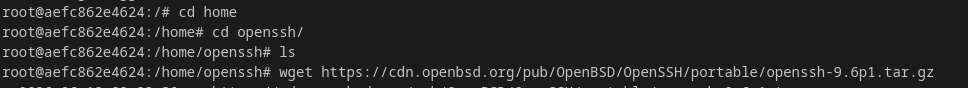
\includegraphics[width=0.9\linewidth]{trafico/01-descarga-openssh.png}
    \caption{Descarga del código fuente de OpenSSH 9.6p1}
\end{figure}

\textbf{Paso 2: Descompresión y acceso al directorio.}
Se descomprimió el archivo descargado con \texttt{tar xzf} y se ingresó al directorio
resultante \texttt{openssh-9.6p1/}.

\begin{figure}[H]
    \centering
    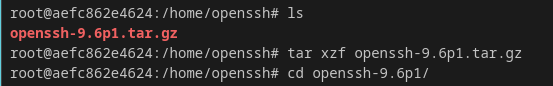
\includegraphics[width=0.9\linewidth]{trafico/02-decompresion-ssh.png}
    \caption{Descompresión del tarball y acceso al directorio fuente}
\end{figure}

\textbf{Paso 3: Apertura del archivo \texttt{version.h} con vim.}
Se abrió el archivo \texttt{version.h} con el editor \texttt{vim} para localizar
la línea que define la cadena de versión del cliente SSH.

\begin{figure}[H]
    \centering
    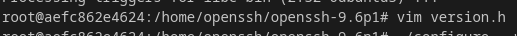
\includegraphics[width=0.9\linewidth]{trafico/03-vim.png}
    \caption{Apertura de version.h con vim}
\end{figure}

\textbf{Paso 4: Modificación de la versión en \texttt{version.h}.}
Se editó la macro \texttt{SSH\_VERSION} cambiando su valor de \texttt{"OpenSSH\_9.6"}
a \texttt{"OpenSSH\_?"}, tal como se observa en la figura. Esta es la cadena que el
cliente enviará durante el handshake SSH.

\begin{figure}[H]
    \centering
    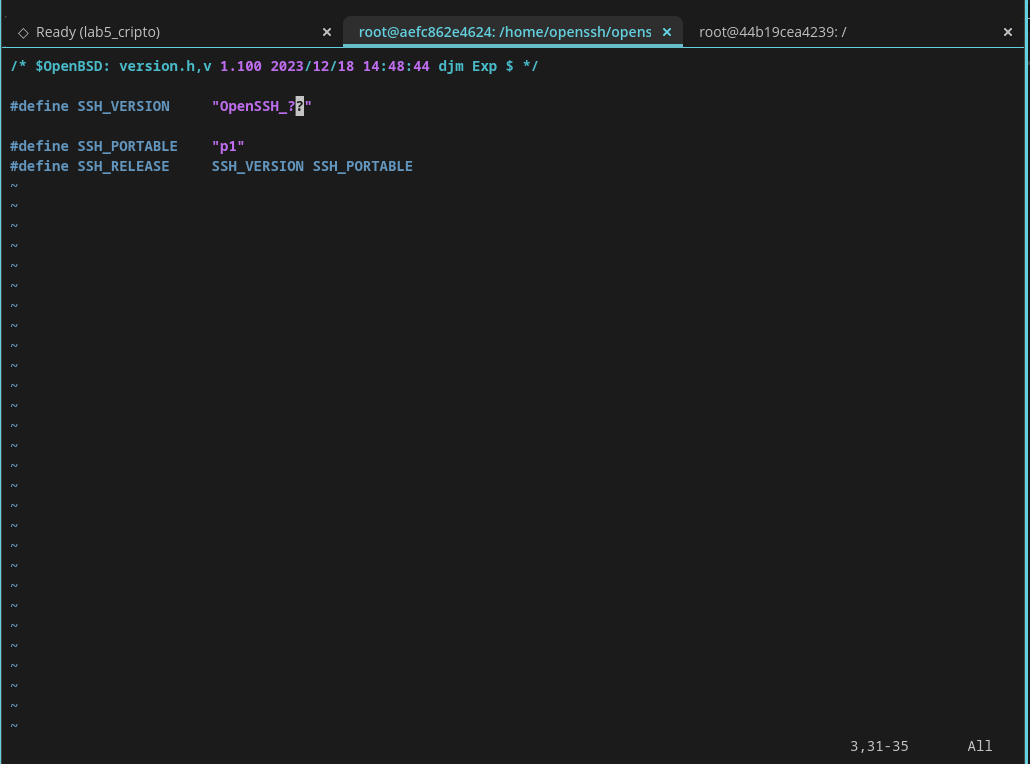
\includegraphics[width=0.9\linewidth]{trafico/04-version.h.png}
    \caption{Modificación de SSH\_VERSION a "OpenSSH\_?" en version.h}
\end{figure}

\textbf{Paso 5: Configuración del entorno de compilación.}
Se ejecutó el script \texttt{./configure} con los parámetros \texttt{--with-pam},
\texttt{--with-zlib} y \texttt{--with-ssl-dir=/usr} para preparar el entorno
de compilación según las librerías disponibles en el contenedor.

\begin{figure}[H]
    \centering
    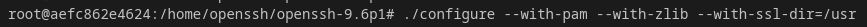
\includegraphics[width=0.9\linewidth]{trafico/05-compilacion1.png}
    \caption{Ejecución de ./configure para preparar la compilación}
\end{figure}

\textbf{Paso 6: Compilación del código fuente.}
Se compiló el proyecto con \texttt{make -j\$(nproc)} para aprovechar todos los
núcleos disponibles y reducir el tiempo de compilación.

\begin{figure}[H]
    \centering
    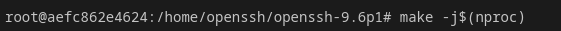
\includegraphics[width=0.9\linewidth]{trafico/06-compilacion2.png}
    \caption{Compilación con make -j\$(nproc)}
\end{figure}

\textbf{Paso 7: Reemplazo del binario y verificación de la versión.}
Se copió el binario compilado sobre \texttt{/usr/bin/ssh} y se verificó con
\texttt{ssh -V} que la versión reportada sea \texttt{OpenSSH\_?p1}. Luego se
realizó la conexión al servidor S1 (\texttt{ssh prueba@172.21.0.10}).

\begin{figure}[H]
    \centering
    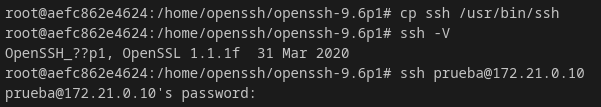
\includegraphics[width=0.9\linewidth]{trafico/07-reemplazoSSH_conection.png}
    \caption{Reemplazo del binario, verificación de versión y conexión al servidor}
\end{figure}

\textbf{Paso 8: Captura del tráfico en Wireshark.}
En la captura se puede observar que el cliente (172.21.0.13) envía al servidor
(172.21.0.10) el paquete de protocolo con el banner \texttt{SSH-2.0-OpenSSH\_??},
confirmando que el tráfico fue replicado exitosamente con la versión \texttt{?}.

\begin{figure}[H]
    \centering
    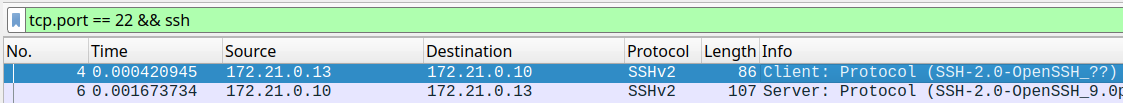
\includegraphics[width=0.9\linewidth]{trafico/08-wireshark.png}
    \caption{Captura Wireshark mostrando el banner SSH-2.0-OpenSSH\_?? en el tráfico replicado}
\end{figure}

\section{Desarrollo (Parte 3)}

\subsection{Replicación del KEI con tamaño menor a 300 bytes (paso por paso)}

El paquete \textit{Key Exchange Init} (KEXINIT) es grande porque contiene listas de
algoritmos separadas por comas para cada categoría: intercambio de llaves, llaves de
host, cifrado, MAC y compresión. El tamaño del paquete es directamente proporcional
a la cantidad de texto en esas listas. Para reducirlo a menos de 300 bytes se modificó
el archivo \texttt{myproposal.h} en el código fuente de OpenSSH dentro del servidor S1,
que es donde se definen esas listas por defecto.

En la imagen se puede observar el archivo antes de la modificación. Las macros
\texttt{KEX\_SERVER\_KEX} y \texttt{KEX\_DEFAULT\_PK\_ALG} contienen largas listas con
9 y 14 algoritmos respectivamente, lo que genera strings de cientos de bytes solo en
esas dos categorías.

\begin{figure}[H]
    \centering
    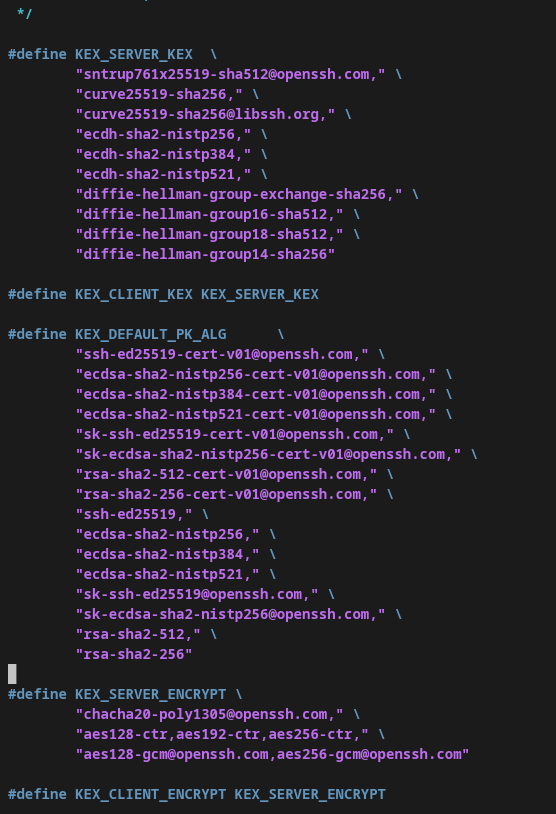
\includegraphics[width=0.85\linewidth]{KEI/myproposal.h.png}
    \caption{Archivo myproposal.h original con las listas completas de algoritmos}
\end{figure}

Se reemplazaron todas las listas por versiones mínimas de un solo algoritmo por
categoría, tal como se ve en la imagen siguiente:

\begin{itemize}
    \item \texttt{KEX\_SERVER\_KEX}: se dejó solo \texttt{diffie-hellman-group14-sha256} (28 bytes)
    \item \texttt{KEX\_DEFAULT\_PK\_ALG}: se dejó solo \texttt{ssh-ed25519-cert-v01@openssh.com} (34 bytes)
    \item \texttt{KEX\_SERVER\_ENCRYPT}: se redujo a \texttt{aes128-ctr,aes192-ctr,aes256-ctr} (31 bytes)
    \item \texttt{KEX\_SERVER\_MAC}: se dejó solo \texttt{hmac-sha2-256} (13 bytes)
\end{itemize}

\begin{figure}[H]
    \centering
    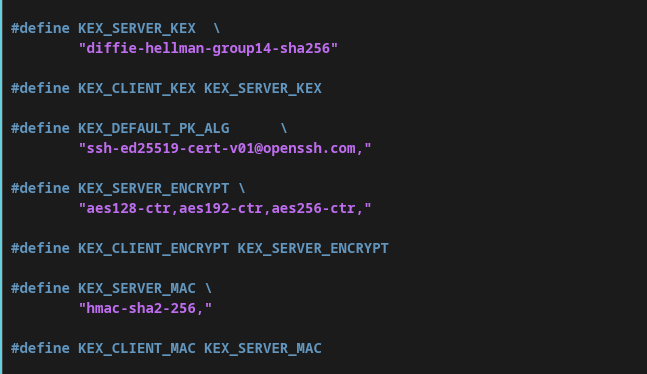
\includegraphics[width=0.85\linewidth]{KEI/myproposal2.png}
    \caption{Archivo myproposal.h modificado con listas mínimas de algoritmos}
\end{figure}

El tamaño del KEXINIT depende directamente del largo de los strings de algoritmos.
Con la configuración original, solo \texttt{KEX\_SERVER\_KEX} ocupa más de 200 bytes.
Al dejar un algoritmo por categoría, la suma total cae a unos 106 bytes, resultando
en un paquete de aproximadamente 168 bytes. Luego se recompiló con \texttt{make sshd}
y se reemplazó el binario en S1.

\section{Desarrollo (Parte 4)}
\subsection{Explicación OpenSSH en general}

OpenSSH es una implementación de código abierto del protocolo SSH (Secure Shell),
diseñada para permitir comunicación remota cifrada entre dos equipos. Opera sobre
TCP, generalmente en el puerto 22. La conexión comienza con un handshake donde
ambos extremos intercambian versiones, negocian algoritmos y generan una llave de
sesión compartida usando Diffie-Hellman o variantes de curvas elípticas. Una vez
establecido el canal cifrado, se realiza la autenticación del usuario (por contraseña
o llave pública) y luego se habilita la sesión.

\subsection{Capas de Seguridad en OpenSSH}

OpenSSH implementa seguridad en tres niveles distintos del protocolo:

\begin{itemize}
    \item Confidencialidad: todo el tráfico se cifra con algoritmos simétricos como
    \texttt{aes128-ctr} o \texttt{chacha20-poly1305}. Nadie que intercepte el tráfico
    puede leer el contenido una vez que el canal está establecido.

    \item Integridad: cada paquete incluye un código de autenticación de mensaje (MAC)
    calculado con algoritmos como \texttt{hmac-sha2-256}. Si el paquete fue modificado
    en tránsito, el receptor lo detecta y descarta la conexión.

    \item Autenticidad: el servidor presenta su llave de host durante el handshake.
    Si el cliente ya conoce esa llave (guardada en \texttt{known\_hosts}), puede
    verificar que está hablando con el servidor correcto y no con un intermediario.
    La autenticación del usuario puede hacerse por contraseña o por par de llaves
    pública/privada.
\end{itemize}

La disponibilidad y el no repudio no son garantizados directamente por el protocolo.
SSH no incluye mecanismos propios contra denegación de servicio, y al autenticarse
por contraseña no existe evidencia criptográfica irrefutable de que fue ese usuario
quien inició sesión, a diferencia de la autenticación por llave pública donde sí
existe esa garantía.

\subsection{Identificación de que protocolos no se cumplen}

A partir del tráfico analizado en este laboratorio, la disponibilidad no se puede
garantizar mediante el protocolo SSH por sí solo, ya que depende de factores externos
como la configuración del servidor y la red. Tampoco se cumple completamente el no
repudio cuando se usa autenticación por contraseña, ya que no existe evidencia
criptográfica que vincule la sesión a una identidad específica. En cambio, con
autenticación por llave pública el no repudio sí se puede argumentar, ya que solo
el poseedor de la llave privada pudo haber firmado el intercambio.

\section*{Conclusiones y comentarios}

En este laboratorio se analizó el comportamiento del protocolo SSH a nivel de tráfico
de red utilizando diferentes versiones de OpenSSH en contenedores Docker. Se comprobó
que cada versión genera una huella digital (HASSH) distinta a partir de los algoritmos
que anuncia en el paquete KEXINIT, lo que permite identificar el cliente con precisión.
Además, se demostró que modificando el código fuente de OpenSSH es posible alterar
tanto la cadena de versión mostrada en el banner como el conjunto de algoritmos
anunciados, logrando reducir el tamaño del KEXINIT del servidor a menos de 300 bytes.
Esto evidencia que la información visible antes del cifrado puede ser manipulada
libremente, lo que tiene implicaciones directas en técnicas de fingerprinting y
en la capacidad de un atacante o analista de inferir información sobre el sistema.

\end{document}
